%% (Master) Thesis template
% Template version used: v1.4
%
% Largely adapted from Adrian Nievergelt's template for the ADPS
% (lecture notes) project.


%% We use the memoir class because it offers a many easy to use features.
\documentclass[11pt,a4paper,titlepage]{memoir}

%% Packages
%% ========

%% LaTeX Font encoding -- DO NOT CHANGE
\usepackage[OT1]{fontenc}

%% Babel provides support for languages.  'english' uses British
%% English hyphenation and text snippets like "Figure" and
%% "Theorem". Use the option 'ngerman' if your document is in German.
%% Use 'american' for American English.  Note that if you change this,
%% the next LaTeX run may show spurious errors.  Simply run it again.
%% If they persist, remove the .aux file and try again.
\usepackage[english]{babel}

%% Input encoding 'utf8'. In some cases you might need 'utf8x' for
%% extra symbols. Not all editors, especially on Windows, are UTF-8
%% capable, so you may want to use 'latin1' instead.
\usepackage[utf8]{inputenc}

%% This changes default fonts for both text and math mode to use Herman Zapfs
%% excellent Palatino font.  Do not change this.
\usepackage[sc]{mathpazo}

%% The AMS-LaTeX extensions for mathematical typesetting.  Do not
%% remove.
\usepackage{amsmath,amssymb,amsfonts,mathrsfs}

%% NTheorem is a reimplementation of the AMS Theorem package. This
%% will allow us to typeset theorems like examples, proofs and
%% similar.  Do not remove.
%% NOTE: Must be loaded AFTER amsmath, or the \qed placement will
%% break
\usepackage[amsmath,thmmarks]{ntheorem}

%% LaTeX' own graphics handling
\usepackage{graphicx}

%% This allows you to add .pdf files. It is used to add the
%% declaration of originality.
\usepackage{pdfpages}

%% For sticking out todo notes and random notes for me
\newcommand{\TODO}[1]{\textcolor{red!60!black}{\textbf{TODO:}~#1}}
\newcommand{\note}[1]{\textcolor{blue!60!red}{~#1}}

%% Some more packages that you may want to use.  Have a look at the
%% file, and consult the package docs for each.
%% See the TeXed file for more explanations

%% [OPT] Multi-rowed cells in tabulars
%\usepackage{multirow}

%% [REC] Intelligent cross reference package. This allows for nice
%% combined references that include the reference and a hint to where
%% to look for it.
\usepackage{varioref}

%% [OPT] Easily changeable quotes with \enquote{Text}
%\usepackage[german=swiss]{csquotes}

%% [REC] Format dates and time depending on locale
\usepackage{datetime}

%% [OPT] Provides a \cancel{} command to stroke through mathematics.
%\usepackage{cancel}

%% [NEED] This allows for additional typesetting tools in mathmode.
%% See its excellent documentation.
\usepackage{mathtools}

%% [ADV] Conditional commands
%\usepackage{ifthen}

%% [OPT] Manual large braces or other delimiters.
%\usepackage{bigdelim, bigstrut}

%% [REC] Alternate vector arrows. Use the command \vv{} to get scaled
%% vector arrows.
\usepackage[h]{esvect}

%% [NEED] Some extensions to tabulars and array environments.
\usepackage{array}

%% [OPT] Postscript support via pstricks graphics package. Very
%% diverse applications.
%\usepackage{pstricks,pst-all}

%% [?] This seems to allow us to define some additional counters.
%\usepackage{etex}

%% [ADV] XY-Pic to typeset some matrix-style graphics
%\usepackage[all]{xy}

%% [OPT] This is needed to generate an index at the end of the
%% document.
%\usepackage{makeidx}

%% [OPT] Fancy package for source code listings.  The template text
%% needs it for some LaTeX snippets; remove/adapt the \lstset when you
%% remove the template content.
\usepackage{listings}

%% Package for algorithms
\usepackage{algorithm2e}

%% [REC] Fancy character protrusion.  Must be loaded after all fonts.
\usepackage[activate]{pdfcprot}

%% [REC] Nicer tables.  Read the excellent documentation.
\usepackage{booktabs}

%% Convert .eps to .pdf for pfdlatex
\usepackage{epstopdf}


%% Our layout configuration.  DO NOT CHANGE.
%% Memoir layout setup

%% NOTE: You are strongly advised not to change any of them unless you
%% know what you are doing.  These settings strongly interact in the
%% final look of the document.

% Dependencies
\usepackage{ETHlogo}

% Turn extra space before chapter headings off.
\setlength{\beforechapskip}{0pt}

\nonzeroparskip
\parindent=0pt
\defaultlists

% Chapter style redefinition
\makeatletter

\if@twoside
  \pagestyle{Ruled}
  \copypagestyle{chapter}{Ruled}
\else
  \pagestyle{ruled}
  \copypagestyle{chapter}{ruled}
\fi
\makeoddhead{chapter}{}{}{}
\makeevenhead{chapter}{}{}{}
\makeheadrule{chapter}{\textwidth}{0pt}
\copypagestyle{abstract}{empty}

\makechapterstyle{bianchimod}{%
  \chapterstyle{default}
  \renewcommand*{\chapnamefont}{\normalfont\Large\sffamily}
  \renewcommand*{\chapnumfont}{\normalfont\Large\sffamily}
  \renewcommand*{\printchaptername}{%
    \chapnamefont\centering\@chapapp}
  \renewcommand*{\printchapternum}{\chapnumfont {\thechapter}}
  \renewcommand*{\chaptitlefont}{\normalfont\huge\sffamily}
  \renewcommand*{\printchaptertitle}[1]{%
    \hrule\vskip\onelineskip \centering \chaptitlefont\textbf{\vphantom{gyM}##1}\par}
  \renewcommand*{\afterchaptertitle}{\vskip\onelineskip \hrule\vskip
    \afterchapskip}
  \renewcommand*{\printchapternonum}{%
    \vphantom{\chapnumfont {9}}\afterchapternum}}

% Use the newly defined style
\chapterstyle{bianchimod}

\setsecheadstyle{\Large\bfseries\sffamily}
\setsubsecheadstyle{\large\bfseries\sffamily}
\setsubsubsecheadstyle{\bfseries\sffamily}
\setparaheadstyle{\normalsize\bfseries\sffamily}
\setsubparaheadstyle{\normalsize\itshape\sffamily}
\setsubparaindent{0pt}

% Set captions to a more separated style for clearness
\captionnamefont{\sffamily\bfseries\footnotesize}
\captiontitlefont{\sffamily\footnotesize}
\setlength{\intextsep}{16pt}
\setlength{\belowcaptionskip}{1pt}

% Set section and TOC numbering depth to subsection
\setsecnumdepth{subsection}
\settocdepth{subsection}

%% Titlepage adjustments
\pretitle{\vspace{0pt plus 0.7fill}\begin{center}\HUGE\sffamily\bfseries}
\posttitle{\end{center}\par}
\preauthor{\par\begin{center}\let\and\\\Large\sffamily}
\postauthor{\end{center}}
\predate{\par\begin{center}\Large\sffamily}
\postdate{\end{center}}

\def\@advisors{}
\newcommand{\advisors}[1]{\def\@advisors{#1}}
\def\@department{}
\newcommand{\department}[1]{\def\@department{#1}}
\def\@thesistype{}
\newcommand{\thesistype}[1]{\def\@thesistype{#1}}

\renewcommand{\maketitlehooka}{\noindent\ETHlogo[2in]}

\renewcommand{\maketitlehookb}{\vspace{1in}%
  \par\begin{center}\Large\sffamily\@thesistype\end{center}}

\renewcommand{\maketitlehookd}{%
  \vfill\par
  \begin{flushright}
    \sffamily
    \@advisors\par
    \@department, ETH Z\"urich
  \end{flushright}
}

\checkandfixthelayout

\setlength{\droptitle}{-48pt}

\makeatother

% This defines how theorems should look. Best leave as is.
\theoremstyle{plain}
\setlength\theorempostskipamount{0pt}

%% This defines how your lstlistings look like
\lstdefinestyle{plain}{%
    language=ML,
    basicstyle={\normalfont\ttfamily},
	tabsize=2,
}

\lstdefinestyle{algorithm}{%
    mathescape,
    basicstyle={\normalfont\small},
	tabsize=2,
	keywordstyle=\textbf,
	otherkeywords={while,if,else,for,end,Input,Output},
	literate={:=}{{$\gets$}}1 {=<}{{$\leq$}}1 {>=}{{$\geq$}}1 {<>}{{$\neq$}}1{->}{$\rightarrow$}1,
}

%%% Local Variables:
%%% mode: latex
%%% TeX-master: "thesis"
%%% End:


%% Theorem environments.  You will have to adapt this for a German
%% thesis.
%% Theorem-like environments

%% This can be changed according to language. You can comment out the ones you
%% don't need.

\numberwithin{equation}{chapter}

%% German theorems
%\newtheorem{satz}{Satz}[chapter]
%\newtheorem{beispiel}[satz]{Beispiel}
%\newtheorem{bemerkung}[satz]{Bemerkung}
%\newtheorem{korrolar}[satz]{Korrolar}
%\newtheorem{definition}[satz]{Definition}
%\newtheorem{lemma}[satz]{Lemma}
%\newtheorem{proposition}[satz]{Proposition}

%% English variants
\newtheorem{theorem}{Theorem}[chapter]
\newtheorem{example}[theorem]{Example}
\newtheorem{remark}[theorem]{Remark}
\newtheorem{corollary}[theorem]{Corollary}
\newtheorem{definition}[theorem]{Definition}
\newtheorem{lemma}[theorem]{Lemma}
\newtheorem{proposition}[theorem]{Proposition}

%% Proof environment with a small square as a "qed" symbol
\theoremstyle{nonumberplain}
\theorembodyfont{\normalfont}
\theoremsymbol{\ensuremath{\square}}
\newtheorem{proof}{Proof}
%\newtheorem{beweis}{Beweis}


%% Helpful macros.
%% Custom commands
%% ===============

%% Special characters for number sets, e.g. real or complex numbers.
\newcommand{\C}{\mathbb{C}}
\newcommand{\K}{\mathbb{K}}
\newcommand{\N}{\mathbb{N}}
\newcommand{\Q}{\mathbb{Q}}
\newcommand{\R}{\mathbb{R}}
\newcommand{\Z}{\mathbb{Z}}
\newcommand{\X}{\mathbb{X}}

%% Fixed/scaling delimiter examples (see mathtools documentation)
\DeclarePairedDelimiter\abs{\lvert}{\rvert}
\DeclarePairedDelimiter\norm{\lVert}{\rVert}

%% Use the alternative epsilon per default and define the old one as \oldepsilon
\let\oldepsilon\epsilon
\renewcommand{\epsilon}{\ensuremath\varepsilon}

%% Also set the alternate phi as default.
\let\oldphi\phi
\renewcommand{\phi}{\ensuremath{\varphi}}


%% Make document internal hyperlinks wherever possible. (TOC, references)
%% This MUST be loaded after varioref, which is loaded in 'extrapackages'
%% above.  We just load it last to be safe.
\usepackage[linkcolor=black,colorlinks=true,citecolor=black,filecolor=black]{hyperref}


%% Document information
%% ====================

\title{Inductive Synthesis from Higher-Order Functions}
\author{Alexandra Maximova}
\thesistype{Master Thesis}
\advisors{Advisors: Prof.\ Dr.\ Martin Vechev, Dimitar Dimitrov}
\department{Department of Computer Science}
\date{August 15, 2016}

\begin{document}

\frontmatter

%% Title page is autogenerated from document information above.  DO
%% NOT CHANGE.
\begin{titlingpage}
  \calccentering{\unitlength}
  \begin{adjustwidth*}{\unitlength-24pt}{-\unitlength-24pt}
    \maketitle
  \end{adjustwidth*}
\end{titlingpage}

%% The abstract of your thesis.  Edit the file as needed.
\begin{abstract}

We investigate the benefits of providing a relatively large library of components to a program synthesiser. Library components encode well-known computational patterns that human programmers reuse in their programs. We target the synthesis of functional straight-line programs from input-output examples. We implement a basic synthesis algorithm based on best-first enumeration combined with type-based pruning. We use heuristics to guide the search and black lists to prune the search space. We have evaluated our prototype implementation on simple algorithmic problems over a library of $37$ components. Results indicate that our basic algorithm performs not considerably worse that much more sophisticated state-of-the-art algorithms.

\end{abstract}


%% TOC with the proper setup, do not change.
\cleartorecto
\tableofcontents
\mainmatter

%% Your real content!
% Some commands used in this file
\newcommand{\package}{\emph}

\chapter{Introduction}\label{ch:introduction}

Let us move on to the contributions. We implemented in OCaml a prototype\footnote{\TODO{Link to the code?}} of the synthesis procedure we define in Chapter~\ref{ch:definitions}. The main contribution of this thesis is the extensive evaluation of our synthesis tool and the exploration of the search space. The experiments and the findings are presented in Chapter~\ref{ch:evaluation}.

The rest of the thesis is structured as follows. In Chapter~\ref{ch:definitions} the top-down synthesis procedure is introduced and formally defined. Chapter~\ref{ch:implementation} describes how to turn this synthesis procedure into a synthesis tool written in OCaml. In Chapter~\ref{ch:relatedwork} we shortly review four closely related synthesis tools: \textsc{Synquid} \cite{SynquidPaper}, $\lambda^2$ \cite{LambdaSquarePaper}, \textsc{Escher} \cite{EscherPaper} and \textsc{Myth} \cite{Mythpaper}. In Chapter~\ref{ch:evaluation} we present the results of the empiric evaluation. Finally, Chapter~\ref{ch:conclusions} draws the conclusions and outlines the possibilities for future work.

\TODO{Write this chapter\\}

\section{What is program synthesis?}

\section{Background}

\section{Problem}
We restrict ourselves to purely functional programs without pattern matching, without recursion, without conditionals, just application of library components and input variables. Handle many components. Reuse common knowledge. Computational patterns encoded as components.






----------------------------------
Plain and simple definition. Program synthesis is the automatic generation of programs. That's what programmers usually do: translate a, mostly oral and ambiguous, specification into a program that satisfies the specification. Wouldn't it be great, if computers once could do the same? (not really, but we leave the ethic and economic reasons out of scope. On the other hand, it would be just like compilers).

What's the problem? Why don't you know what to write in this chapter? It shouldn't be that difficult. You need
\begin{itemize}
\item general introduction/motivation. Don't forget to say what is program synthesis. "What is program synthesis"
\item background section "The problem is too general. Other restricted it in this and this way, tried this and this approach. Logical specification and deduction, input-output examples and induction, restrict to a particular domain like sketch and the bit-manipulating things or igor for number series. flashfill in excel gibt es auch noch. For functional programs we have this and this approaches and this and this restrictions"
\item intuitive description of the problem statement and a motivation why something that restricted should be interesting (encode computational patterns as components, thin interfaces, SKI as components). Bring the replicate example. Type-driven, example-based, from components. Should be stated clearly. "How I restrict the search space and what specification do I choose. Replicate example. Motivate why it could be useful and why this is not too restricted." Don't forget the main hypothesis, that higher-order components help.
\item list of contributions (what are my contributions? The algorithm is standard, the implementation is not really a contribution. Evaluation? Should I stress that this is empirical work?) "Move on to the contributions. Implementation and extensive empirical evaluation".
\item structure of the thesis (formal definition of the synthesis procedure, implementation, four closely related tools, evaluation). Well, you know how to write those sections :)
\end{itemize} 


Unlike our synthesis procedure, all of these tools are capable of synthesising recursive programs. This is not really a limitation, since common recursive patterns can be encoded as components. For example, the program \lstinline!p n = foldNatNat f init n! can be translated into the recursive program
\TODO{Make sure it is \lstinline!f (n-1) (p (n-1))! and not \lstinline!f n (p (n-1))!, correct if needed\\}
\begin{lstlisting}[style=plain]
p n = match n with
  | 0 -> init
  | n -> f (n-1) (p (n-1))
\end{lstlisting}  

for motivation you could write something about the extremely restricted list library in ocaml :)\\
Consider you are writing code in a functional programming language with a smaller choice of library functions than you are used to. For example (true story), if you are using OCaml and you are surprised that \lstinline?replicate? is missing even in the more complete core library \note{cite jane street core}, you could spend a couple of minutes writing your recursive version of \lstinline?replicate?. Or you can synthesize it with \textsc{Tamandu} in less than one second from other components. \TODO{rewrite without 'you' and maybe don't mention ocaml, core and all that thing?}.

input-output examples are an intuitive and simple way to specify programs and make synthesis more accessible to users with a lower level of expertise.


Problem definition: have many components, put them together into a program, no lambdas, no if-then-else, no recursion
  

  
  
Contributions: Evaluation, exploring the baseline algorithm, exploring the search space

\lstset{style=plain}

\chapter{Related Work} \label{ch:relatedwork}

In this chapter we look at four state-of-the-art tools closely related to our work. They all synthesise functional programs, are based on inductive enumeration and use type information to restrict the search space. Since simple types are too ambiguous to specify a program, the tools we present either choose to complement type information with input-output examples or resort to more complex and more expressive types that can actually act as a specification, as for example the \emph{refinement types} from \cite{SynquidPaper}.

\section{\mdseries\textsc{Synquid}}

In \cite{SynquidPaper} \textsc{Synquid} is proposed. The code can be found online\footnote{https://bitbucket.org/nadiapolikarpova/synquid} and there is the possibility to try it in the browser.
This tool uses \emph{refinement types} (types decorated with logical predicates) to prune the search space and to specify programs. SMT-solvers are used to satisfy the logical predicates appearing in the types.\\
Refinement types were already successfully used for verification. In particular, the tool builds upon the liquid types framework \cite{LiquidTypes}. However, it proposes a new procedure for type inference (called modular refinement type reconstruction), which thank to its modularity scales better than other existing inference procedures for refinement types. Programs can therefore be type checked even before they are put together.

This tool targets a language that includes lambda expressions, pattern matching, structural recursion, conditionals and fixpoint.
The user can define custom functions and inductive datatypes that can be passed to the synthesiser as components.

A program is specified by providing a type signature. For example, the synthesis goal \lstinline!replicate! can be specified as follows.
\begin{lstlisting}[style=plain]
n : Nat -> x : $\alpha$ -> {List $\alpha$ | len $\nu$ = n}
\end{lstlisting}
This is a dependent function type that denotes functions that, given a natural number $n$ and an $x$ of type $\alpha$, return a list of $\alpha$ of length $n$. Here $\nu$ is a special logical value variable that in this case denotes the runtime return value of the functions and \lstinline!len! is a measure function defined over lists.

This form of specification can be a disadvantage, since it is not that accessible to users with a lower level of expertise as input-output examples. It is not always easy to see which measure function for a custom datatype will lead to the most simple and intuitive specification.
On the other hand, refinement types allow to express programs that manipulate data structures with non-trivial universal and inductive invariants in a concise way. This allows to synthesise programs on sorted lists, unique lists, binary search trees, heaps and red-black trees.

This tool synthesises simple programs over lists and integers in under \SI{0.4}{s}. It can also handle more complex benchmarks that are out of the scope of this thesis, such as different sorting algorithms and manipulations of data structures with complex invariants. Various sorting algorithms over lists and trees are synthesised in under \SI{5}{s}. The synthesis of the most complex benchmark, the balancing of a red-black tree, takes up to \SI{20}{s}.

In contrast to our tool, the number of components provided to the synthesiser for evaluation is small.

\section{$\lambda^2$}
The tool proposed in \cite{LambdaSquarePaper} is called $\lambda^2$ and generates its output in $\lambda$-calculus with algebraic types and recursion. The target language also includes $7$ higher-order combinators such as \lstinline!map!, \lstinline!fold! and \lstinline!filter! and a flexible set of primitive operators and constants.

The user specifies the desired program providing only input-output examples. No particular knowledge is required from the user, as was demonstrated using randomly generated input-output examples. The goal type is inferred from the examples.

The synthesis algorithm is a combination of inductive generalisation, a limited form of deduction and enumerative search.
First, it generates \emph{hypotheses} in a type-aware manner, that is programs with free variables such as \lstinline!$\lambda$x. map ?f x! where \lstinline!?f! is a placeholder for an unknown program to be synthesised.
Then deduction in form of hand-coded rules about the higher-order combinators is used either to refute a hypothesis or infer new input-output examples to guide the synthesis of missing functions. For example, the hypothesis \lstinline!$\lambda$x. map ?f x! will be refuted if the length of the input list does not match the length of the output length.
Enumerative search is used to enumerate candidate programs to fill in the missing parts of hypotheses. Hypotheses and candidate programs are organised in a priority queue and, at each point of the search, the least-cost candidate is picked.

This tool is able to synthesize programs manipulating recursive data structures like lists, trees and nested data structures such as lists of lists and trees of lists.
It synthesises all benchmark programs in under 7~minutes. Half of the benchmarks is synthesised in under \SI{0.43}{s}. However, the synthesis of \lstinline!droplast!, the program that drops the last element of a list, takes up to \SI{320}{s}. The program that removes duplicates from a list, the program that drops the smallest elements of each list of a list of lists and the program that inserts a tree under each leaf of another tree take more than \SI{100}{s} to synthesise.

Unlike \textsc{Synquid} and our work, this tool can only use the $7$ hard-coded higher-order combinators. The extension of the set of higher-order combinators with own functions is not easily supported.


\section{\mdseries\textsc{Escher}}

In \cite{EscherPaper} \textsc{Escher} is presented. This tool targets a simple untyped purely functional language consisting of constants, input variables, conditionals and library components applied to all of their arguments, including a special component \lstinline!self! referring to the program being synthesised. This last component is used to synthesise recursive programs.

The user specifies the desired program as a \emph{closed} set of input-output examples. That is, for each input-output example, all examples needed to evaluate every recursive call must be present. For example, if we want to specify \lstinline!replicate! as
\begin{lstlisting}[style=plain]
replicate 2 'a' = ['a','a'],
\end{lstlisting}
we also need to provide the input-output examples for the possible recursive calls, that is
\begin{lstlisting}[style=plain]
replicate 1 'a' = ['a']
replicate 0 'a' = [].
\end{lstlisting}
This is necessary because recursive programs are evaluated using the input-output examples as an oracle. However, it is not always easy for an inexperienced user to provide such a set.

The search is goal-directed. Programs are associated with value vectors, that is the vector of the outputs of the program on the inputs from the input-output examples. Programs sharing the same value vectors are considered equivalent, that is the search space is pruned based on observational equivalence.
The algorithm alternates between two phases: forward search and conditional inference. During forward search programs are inductively enumerated by adding new components to already synthesised programs. During conditional inference a novel data structure, the \emph{goal graph}, is used to detect when two synthesised programs can be joined by a conditional statement. The alternation between the two phases is guided by a heuristic.

This tool is able to synthesise recursive programs, including tail recursive, mutually recursive and divide-and-conquer. It synthesises all benchmarks in under \SI{11}{s} and all but three benchmarks in under \SI{1}{s}. The benchmarks include programs on integers such as \lstinline!fibonacci! and \lstinline!isEven!, programs on lists such as \lstinline!compress! and \lstinline!insert! and programs on trees such as \lstinline!nodes-at-level! and \lstinline!count-leaves!.

Like our work, this tool can handle a flexible set of components. For example, a set of $23$ components was used to evaluate all benchmarks. However, there was no higher-order component among them.

\section{\mdseries\textsc{Myth}}
\TODO{Write this section\\}
Myth (Osera). Like mine, requires type and I/O-examples. Refinement tree.
\begin{enumerate}
\item What is the specification?
A type signature, the components and a list of input-output examples.
\item What is the target language?
pattern matching, recursion, higher-order functions in typed programming languages. Can synthesise higher-order functions, programs using higher-order functions and work with large algebraic datatypes.
ML-like language with algebraic data types, match, top-level function definitions and explicitly recursive functions.
\item What can they do well and fast? How fast?
Recursive programs with pattern matching. It's very fast, many programs are synthesised in around 0.1~s. It can also generate larger programs (75 AST nodes) in reasonable time (3~s for calculating the set of free variables in an untyped lambda-calculus).
\item What is the difficulty? What can they not generate (or take a long time)? How much time do they need?
To generate recursive functions, they also need a closed set of examples, so that a recursive call to the function being synthesised can be answered by an input-output example. They also require relatively many examples. They use a relatively large context, but they do not say how big it is.
Lacks support richer types like products and polymorphic types.
\item What do they do?
The tool in \cite{MythPaper} is called \textsc{Myth} and uses not only type information but also input-output examples to restrict the search space. The special data structure used to hold this information is the \emph{refinement tree}. This system can synthesize higher-order functions, programs that use higher order functions and work with large algebraic data types.\\
There is an ML-like type system that incorporates input-output examples. Two pieces: a \emph{refinement tree} and an enumerative search.\\
Two major operations: refine the goal type and the examples (push them down in the refinement tree) and guess a term of the right type that matches the examples (for one of the nodes of the refinement tree).\\
\end{enumerate}





%Leon (can bring it, it's deductive, so it's different than the others. It also targets functional programs. No, I have nothing to compare. The benchmark is too different.) \cite{LeonPaper}
%\begin{enumerate}
%\item What is the specification?
%Input-output relations (including examples), pre- and postconditions.
%\item What is the target language?
%Several recursion schemas (only terminating programs), components, pattern matching
%\item What can they do well and fast? How fast?
%The good thing is that they generate verified software. And it's interactive, the user can control the structure if he wants to.
%\item What is the difficulty? What can they not generate (or take a long time)? How much time?
%
%\item What do they do?
%Deductive synthesis, counterexample-guided.
%That's from the verification side: the point is to deliver \emph{verified} software that satisfies some specifications such as assertions, pre-conditions and post-conditions.
%\end{enumerate}


%%% Local Variables:
%%% mode: latex
%%% TeX-master: "thesis"
%%% End:

\chapter{Benchmarks} \label{benchmarks}

\note{
Some programs over numbers, some over lists, some over lists of lists and some over trees (What kind of trees?).
For every program, try to get a sample implementation. \\
Types needed: \lstinline?Int, [a], Tree a? \\
Basic components needed:
arithmetic (\lstinline?+, -, *, /?), 
relation (\lstinline?<, <=, ==, /=, >=, >?),
\note{(maybe we do not need relations)}
}

\begin{enumerate}
	\item max of two numbers\\
	(hopefully) the easiest program \\
	\begin{lstlisting}
max :: Int -> Int -> Int
max 0 0 == 0
max 1 0 == 1
max 0 1 == 1
max x y = if x > y then x else y
	\end{lstlisting}
	\note{We don't care about conditionals, we cannot synthesize this.}\\
	This is the only function that requires a conditional branch.
%
	\item square a number
	\begin{lstlisting}
square :: Int -> Int -> Int
square 0 == 0
square 1 == 1
square 2 == 4
square 3 == 9
square x = x * x
	\end{lstlisting}
	That is, basic arithmetic operations like \lstinline!+ - * /! should be provided
%
	\item tetrahedral numbers \\
	\begin{lstlisting}
tetrahedral :: Int -> Int
tetrahedral 1 == 1
tetrahedral 2 == 4
tetrahedral 3 == 10
	\end{lstlisting}
	closed form solution
	\begin{lstlisting}
tetrahedral n = n * (n+1) * (n+2) / 6
	\end{lstlisting}
	iterative solution
	\begin{lstlisting}
tetrahedral n = scanl1 (+) (scanl1 (+) [0..]) !! n
	\end{lstlisting}
	Another iterative solution (without infinite lists)
	\begin{lstlisting}
tetrahedral n = foldl1 (+) (scanl1 (+) (enumFromTo 1 n))
	\end{lstlisting}
	Components needed: \lstinline?scanl1, !!? \\
	Interestingly the iterative version is much faster than the closed form solution
%
	\item prime test \\
	I think this is too difficult
	\begin{lstlisting}
prime :: Int -> Int
prime 1 == 0
prime 2 == 1
prime 3 == 1
prime 4 == 0
prime 25 == 0
prime 29 == 1
prime n = minimum (1 : (map (mod n) (enumFromTo 2 (subtract 1 n))))
	\end{lstlisting}
	Components needed: \lstinline?map, mod, minimum, enumFromTo, subtract?
%
	\item average
	\begin{lstlisting}
average :: [Int] -> Int
average [1] == 1
average [1,3] == 2
average [1,2,3,6] == 6
average xs = (sum xs) `div` (length xs)
	\end{lstlisting}
%
	\item movingAverage (forward)
	\begin{lstlisting}
movingAverage :: Int -> [Int] -> [Int]
movingAverage 1 [1,2,3] == [1,2,3]
movingAverage 2 [1,2,3] == [2,2,3]
movingAverage 3 [3,2,4,1,5,2] == [3,2,3,2,3,2]
movingAverage n xs = map (average . take n) (init $ tails xs)
	\end{lstlisting}
	Components needed: \lstinline?tails? from \lstinline?Data.List? and  \lstinline?average? (one of the benchmarks), as well as \lstinline?map, take? and \lstinline?init? from \lstinline?Prelude?.
%
	\item movingSum (backward)
	\begin{lstlisting}
movingSum :: Int -> [Int] -> [Int]
movingSum 1 [1,2,3] == [1,2,3]
movingSum 2 [1,2,3] == [1,3,5]
movingSum 3 [4,8,6,-1,-2,-3,-1,3,4,5] == [4,12,18,13,3,-6,-6,-1,6,12]
movingSum n xs = scanl1 (+) (zipWith (-) xs (replicate n 0 ++ xs))
	\end{lstlisting}
%
	\item waterflow problem \\
	Given an array of "wall" heights, determine the volume of the puddles that can form if it rains.
	\begin{lstlisting}
water :: [Int] -> Int
water [1,2,3] == 0
water [5,2,5] == 3
water [2,3,1,6,1] == 2
water h = sum $ 
      zipWith (-) 
        (zipWith min (scanl1 max h) (scanr1 max h))
        h
	\end{lstlisting}
%
	\item horner schema to evaluate polynomials
	\begin{lstlisting}
horner :: [Int] -> Int -> Int
horner [1,2,3] 1 == 6
horner [1,2,3] 2 == 11
horner [4,3,2] 3 == 47
horner p x = foldl1 ((+) . (x *)) p
	\end{lstlisting}
	Problem: we do not generate lambda's. Do we generate functions like \lstinline?(x *)??
%
	\item sum-under, sum all integers up to the argument
	\begin{lstlisting}
sum_under :: Int -> Int
sum_under 0 == 0
sum_under 1 == 1
sum_under 2 == 3
sum_under 3 == 6
sum_under 4 == 10
sum_under n = sum [1..n]
	\end{lstlisting}
	Components needed: \lstinline?sum, enumFromTo?
%
	\item factorial \\
	\begin{lstlisting}
factorial :: Int -> Int
factorial 0 == 0
factorial 1 == 1
factorial 3 == 6
factorial 5 == 120
factorial n = product [1..n]
	\end{lstlisting}
	interesting for intermediate states
%
	\item maximum of a list\\
	I don't know (yet) how to specify a "global property" like greater or smaller than all other elements in a list in \textsc{Synquid}. Moreover, it seems a difficult property to extract from input-output examples.
	\begin{lstlisting}
maximum :: [Int] -> Int
maximum [1,3,2] == 3
maximum [4,2,1] == 4
maximum [1,3,5] == 5
maximum xs = foldr max (head xs) xs
	\end{lstlisting}
	Or just use the \lstinline?maximum? function from \lstinline?Prelude?, if it is given as a component
%
	\item append two lists\\
	The specification given by Nadia does not synthesize the usual append function. Maybe it's better to let her know...\\
	Although it's possible to synthesize append in \textsc{Synquid}.
	\begin{lstlisting}
append :: [a] -> [a] -> [a]
append [1,2,3] [4,5,6] == [1,2,3,4,5,6]
append [1,2] [6,2,3] == [1,2,6,2,3]
append xs ys = foldr (:) ys xs
	\end{lstlisting}
	Or use \lstinline?++? from \lstinline?Prelude?, if we decide to provide it for this example too.
%
	\item length of a list \\
	Can be also interesting for intermediate states
	\begin{lstlisting}
length :: [a] -> Int
length [1,2,3] == 3
length [2,2,2] == 3
length [] == 0
length [5] == 1
length xs = sum $ map (const 1) xs
	\end{lstlisting}
%
	\item list reversal
	\begin{lstlisting}
reverse :: [a] -> [a]
reverse [1,2,3] == [3,2,1]
reverse [5,2,3] == [3,2,5]
reverse [6,2,3,1] == [1,3,2,6]
reverse xs = foldl (flip (:)) [] xs
	\end{lstlisting}
%
	\item bagsum: \lstinline![far,bar,gar,bar,bar,far] -> [(bar,3),(far,2),(gar,1)]!\\
	Seems difficult and maybe intermediate states can be helpful. Should I take \lstinline?Int? instead of \lstinline?a?? I mean, \lstinline?a? should belong to the typeclass \lstinline?Ord?, otherwise we cannot yield a sorted output list. And we do not have any other base types anyway. But actually lists of integers are also ordable. Hence also lists of lists of integers and lists of lists of lists of integers and so on.
	\begin{lstlisting}
bagsum :: [a] -> [(a, Int)]
bagsum [1,1,1] == [(1,3)]
bagsum [4,4,2,1,2,1] == [(1,2),(2,2),(4,2)]
bagsum [3,2,1,3,2,3] == [(1,1),(2,2),(3,3)]
bagsum xs = map (head &&& length) (group (sort xs))
	\end{lstlisting}
	Components needed: \lstinline?&&&? from \lstinline?Control.Arrow?. And we also need \lstinline?Tuples? for this one.
%
	\item map \\
	Isn't it a higher order function? I thought we synthesize only first order functions.\\
	How can we provide examples? I mean, we have to write functions as well.\\
	\begin{lstlisting}
map :: (a -> b) -> [a] -> [b]
map f xs = foldr ((:) . f) [] xs
	\end{lstlisting}
%
	\item zipWith \\
	it's a higher order function as well. We need Tuples.\\
	How do we provide the examples?
	\begin{lstlisting}
zipWith :: (a -> b -> c) -> [a] -> [b] -> [c]
zipWith f xs ys = map (uncurry f) (zip xs ys)
	\end{lstlisting}
	Components needed: \lstinline?map, uncurry, zip?.
%
	\item list drop
	\begin{lstlisting}
drop :: Int -> [a] -> [a]
drop 0 [1,2,3] == [1,2,3]
drop 1 [1,2,3] == [2,3]
drop 5 [5,4,2,5] == []
drop 3 [4,2,3,1] == [1]
drop n xs = snd (splitAt n xs)
	\end{lstlisting}
%
	\item droplast, drop the last element of a list
	\begin{lstlisting}
droplast :: [a] -> [a]
droplast [] == []
droplast [1] == []
droplast [1,2,3] == [1,2]
droplast [3,2,1]== [3,2]
droplst = init
droplast' xs = map fst (zip xs (enumFromTo 1 (subtract 1 (length xs))))
droplast'' xs = take (subtract 1 (length xs)) xs
	\end{lstlisting}
%
	\item dropmax, drop the greatest element of a list\\
	$\lambda^2$ takes much more time to synthesize droplast than dropmax. Why?
	\begin{lstlisting}
dropmax :: [Int] -> [Int]
dropmax [1,2] == [1]
dropmax [2,1] == [1]
dropmax [1,2,3] == [1,2]
dropmax [3,2,1] == [2,1]
dropmax [2,3,1] == [2,1]
dropmax xs = filter (/= (maximum xs)) xs
	\end{lstlisting}
%
	\item dedup, remove duplicates from a list \\
	$\lambda^2$ requires more time\\
	\TODO{Find a non-recursive implementation that preserves the order of the elements} Either implement it with \lstinline?groupBy? or say you cannot implement it. Say it's not possible to get the usual semantics of deleting all but the first occurrence of some program.
%
	\item sort by length (on lists of lists)
	\begin{lstlisting}
sortByLength :: [[a]] -> [[a]]
sortByLength [[1,2],[1,2,3],[1]] == [[1],[1,2],[1,2,3]]
sortByLength = sortBy (curry ((uncurry compare) . (length *** length)))
	\end{lstlisting}
	\TODO{Is there a shorter implementation?} What's wrong with this one? \\
	Components needed: \lstinline?(***)? from \lstinline?Control.Arrow?
%
	\item dropmins \\
	$\lambda^2$ required more time to synthesize it
	\begin{lstlisting}
dropmins :: [[Int]] -> [[Int]]
dropmins [[1,2,3],[2,3,1],[2,3],[1]] == [[2,3],[2,3],[3],[]]
dropmins = map dropmin
	\end{lstlisting}
	\TODO{Is there an implementation without the auxiliary function \lstinline?dropmin? and without lambda expressions?} Yes, there is one, but you don't want to see it. With \lstinline?ap? and \lstinline?join?.
%
	\item lasts, last element of every list \\
	another program on nested lists
	\begin{lstlisting}
lasts :: [[a]] -> [a]
lasts [[1,2,3],[3,2],[4,2,4,1],[2]] == [3,2,1,2]
lasts = map last
	\end{lstlisting}
%
	\item member of the tree\\
	Something with trees. Membership seems a difficult thing to learn from input-output examples.
%
	\item count leaves it a tree
%
	\item nodes at level
	The standard Haskell tree is a rose tree. Defined in \lstinline?Data.Tree?.
	
\note{Nadia has more complicated examples with Red-Black-Trees, AVL-trees and different sorting algorithms}
\end{enumerate}




%%% Local Variables:
%%% mode: latex
%%% TeX-master: "thesis"
%%% End:


\appendix

\chapter{Dummy Appendix}

You can defer lengthy calculations that would otherwise only interrupt
the flow of your thesis to an appendix.


\backmatter

\bibliographystyle{plain}
\bibliography{refs}

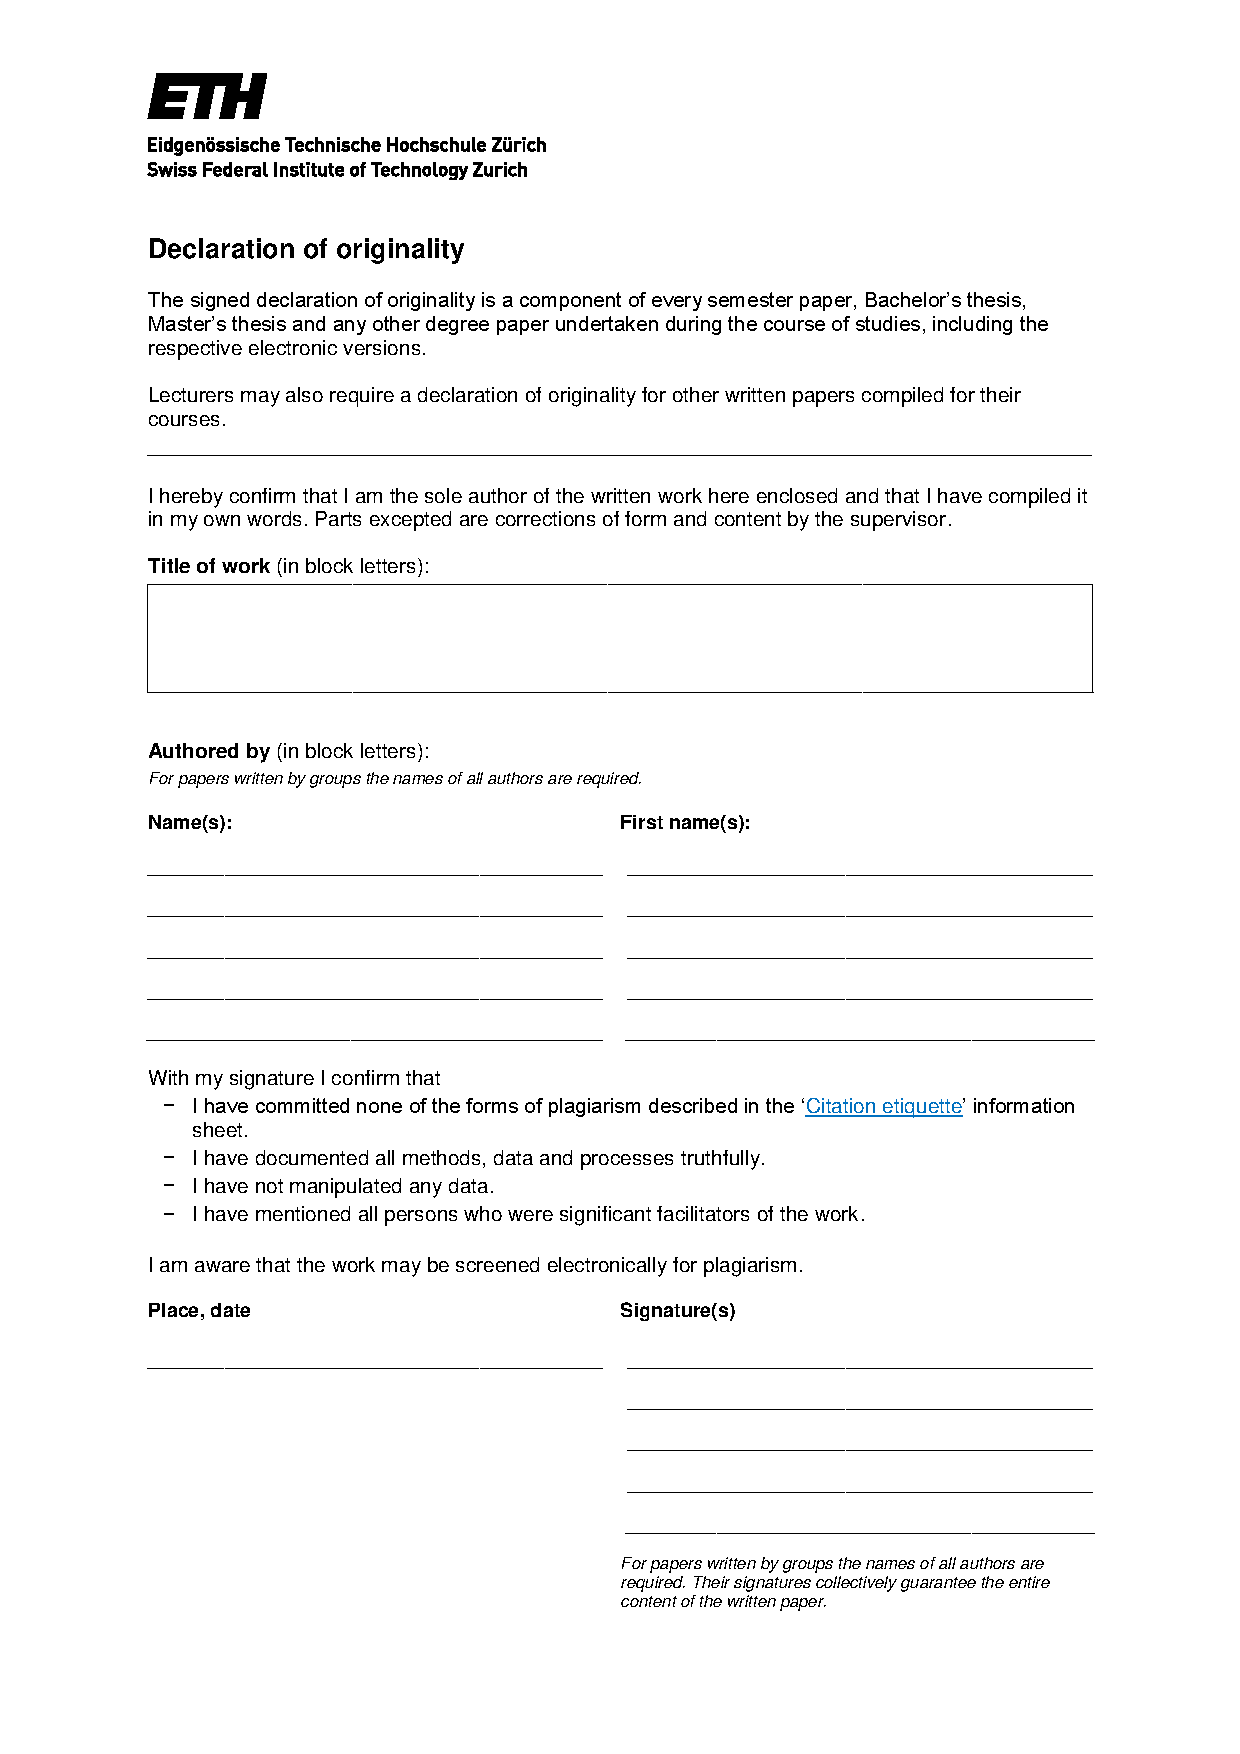
\includepdf[pages={-}]{declaration-originality.pdf}

\end{document}
